\documentclass[11pt]{article}

% Shared notes settings for Applied Machine Learning lectures (UPES).
% Keep this file free of \documentclass to allow reuse via \input.

\usepackage[utf8]{inputenc}
\usepackage[T1]{fontenc}
\usepackage{lmodern}          % scalable T1 fonts; without this pdflatex falls back
\input{glyphtounicode}        % to bitmapped EC Type 3 and the PDFs are neither
\pdfgentounicode=1            % searchable nor screen-reader friendly
\usepackage[a4paper,margin=1in]{geometry}
\usepackage{hyperref}
\usepackage{xurl}
\usepackage{booktabs}
\usepackage{amsmath}
\usepackage{amssymb}
\usepackage{listings}
\usepackage{xcolor}
\usepackage{enumitem}
\usepackage{parskip}

% Code listings (Python-oriented for this subject).
\lstset{
  language=Python,
  basicstyle=\ttfamily\small,
  keywordstyle=\color{blue},
  commentstyle=\color{gray},
  stringstyle=\color{teal},
  showstringspaces=false,
  columns=fullflexible,
  frame=single,
  framerule=0.2pt,
  breaklines=true
}

\setlist[itemize]{topsep=0.3em,itemsep=0.2em}
\setlist[enumerate]{topsep=0.3em,itemsep=0.2em}

% Simple per-section source line.
\newcommand{\notesources}[1]{\par\noindent{\small\color{gray}\textit{Sources:} \sloppy #1\par}}

% Unit-wise source strings for this subject (used by slides + notes).
% Path is relative to the lecture `latex/` folder (the compilation CWD).
\IfFileExists{../../../_shared/aml-sources.tex}{%
  % Source strings for Applied Machine Learning (CSAI2017P) — used by slides + notes.
% Prescribed texts and reference books are taken from the course syllabus.
% Support texts are the author-hosted open-access editions:
%   statlearning.com            (ISL with Python)
%   probml.github.io/pml-book   (Murphy, Probabilistic Machine Learning)
%   d2l.ai                      (Dive into Deep Learning)
%   mml-book.github.io          (Mathematics for Machine Learning)

\newcommand{\AMLRepoURL}{https://github.com/tali7c/Applied-Machine-Learning}

% --- prescribed -------------------------------------------------------------
\newcommand{\AMLPrescribed}{%
M\"uller and Guido, \textit{Introduction to Machine Learning with Python}, O'Reilly, 2016.;%
Bishop, \textit{Pattern Recognition and Machine Learning}, Springer, 2006.;%
Murphy, \textit{Machine Learning: A Probabilistic Perspective}, MIT Press, 2012.;%
Han, Kamber and Pei, \textit{Data Mining: Concepts and Techniques} (3e), Morgan Kaufmann, 2012.%
}

% --- unit-wise ---------------------------------------------------------------
\newcommand{\AMLUnitISources}{%
M\"uller and Guido, \textit{Introduction to Machine Learning with Python}, Ch. 1.;%
Bishop, \textit{Pattern Recognition and Machine Learning}, Ch. 1.;%
Murphy, \textit{Probabilistic Machine Learning: An Introduction}, MIT Press, 2022, Ch. 1.;%
Mitchell, \textit{Machine Learning}, McGraw Hill, 1997, Ch. 1.;%
Scikit-learn documentation, accessed 2026-08-04.%
}

\newcommand{\AMLUnitIISources}{%
Bishop, \textit{Pattern Recognition and Machine Learning}, \S1.5, \S4.3, \S7.1.;%
Zhang, Lipton, Li and Smola, \textit{Dive into Deep Learning}, \S3.4.;%
Shalev-Shwartz and Ben-David, \textit{Understanding Machine Learning}, Ch. 15.;%
Murphy, \textit{Probabilistic Machine Learning: An Introduction}, Ch. 5.%
}

\newcommand{\AMLUnitIIISources}{%
Zhang, Lipton, Li and Smola, \textit{Dive into Deep Learning}, Ch. 12 (Optimization Algorithms).;%
Deisenroth, Faisal and Ong, \textit{Mathematics for Machine Learning}, Ch. 7.;%
Kingma and Ba, ``Adam: A Method for Stochastic Optimization,'' ICLR 2015.;%
Ruder, ``An overview of gradient descent optimization algorithms,'' arXiv:1609.04747, 2016.%
}

\newcommand{\AMLUnitIVSources}{%
Han, Kamber and Pei, \textit{Data Mining: Concepts and Techniques} (3e), Ch. 3.;%
M\"uller and Guido, \textit{Introduction to Machine Learning with Python}, Ch. 3--4.;%
James, Witten, Hastie, Tibshirani and Taylor, \textit{An Introduction to Statistical Learning with Python}, Ch. 5--6, 12.;%
Scikit-learn documentation (preprocessing, model selection), accessed 2026-08-04.%
}

\newcommand{\AMLUnitVSources}{%
James et al., \textit{An Introduction to Statistical Learning with Python}, Ch. 3--6.;%
Bishop, \textit{Pattern Recognition and Machine Learning}, Ch. 3.;%
Deisenroth, Faisal and Ong, \textit{Mathematics for Machine Learning}, Ch. 9.;%
M\"uller and Guido, \textit{Introduction to Machine Learning with Python}, \S2.3.%
}

\newcommand{\AMLUnitVISources}{%
Han, Kamber and Pei, \textit{Data Mining: Concepts and Techniques} (3e), Ch. 8--9.;%
James et al., \textit{An Introduction to Statistical Learning with Python}, Ch. 8--9.;%
Bishop, \textit{Pattern Recognition and Machine Learning}, Ch. 4--5, 7, 14.;%
Zhang et al., \textit{Dive into Deep Learning}, Ch. 5.%
}

\newcommand{\AMLUnitVIISources}{%
Han, Kamber and Pei, \textit{Data Mining: Concepts and Techniques} (3e), Ch. 10.;%
James et al., \textit{An Introduction to Statistical Learning with Python}, Ch. 12.;%
M\"uller and Guido, \textit{Introduction to Machine Learning with Python}, \S3.5.;%
Ester, Kriegel, Sander and Xu, ``A density-based algorithm for discovering clusters (DBSCAN),'' KDD 1996.%
}

\newcommand{\AMLLabSources}{%
M\"uller and Guido, \textit{Introduction to Machine Learning with Python}, companion notebooks.;%
McKinney, \textit{Python for Data Analysis} (3e), O'Reilly, 2022.;%
Scikit-learn user guide, accessed 2026-08-04.;%
Matplotlib and Seaborn documentation, accessed 2026-08-04.%
}
%
}{%
  % Faculty copies live under `private/` so their compile CWD is different.
  \IfFileExists{../../../../public/_shared/aml-sources.tex}{%
    % Source strings for Applied Machine Learning (CSAI2017P) — used by slides + notes.
% Prescribed texts and reference books are taken from the course syllabus.
% Support texts are the author-hosted open-access editions:
%   statlearning.com            (ISL with Python)
%   probml.github.io/pml-book   (Murphy, Probabilistic Machine Learning)
%   d2l.ai                      (Dive into Deep Learning)
%   mml-book.github.io          (Mathematics for Machine Learning)

\newcommand{\AMLRepoURL}{https://github.com/tali7c/Applied-Machine-Learning}

% --- prescribed -------------------------------------------------------------
\newcommand{\AMLPrescribed}{%
M\"uller and Guido, \textit{Introduction to Machine Learning with Python}, O'Reilly, 2016.;%
Bishop, \textit{Pattern Recognition and Machine Learning}, Springer, 2006.;%
Murphy, \textit{Machine Learning: A Probabilistic Perspective}, MIT Press, 2012.;%
Han, Kamber and Pei, \textit{Data Mining: Concepts and Techniques} (3e), Morgan Kaufmann, 2012.%
}

% --- unit-wise ---------------------------------------------------------------
\newcommand{\AMLUnitISources}{%
M\"uller and Guido, \textit{Introduction to Machine Learning with Python}, Ch. 1.;%
Bishop, \textit{Pattern Recognition and Machine Learning}, Ch. 1.;%
Murphy, \textit{Probabilistic Machine Learning: An Introduction}, MIT Press, 2022, Ch. 1.;%
Mitchell, \textit{Machine Learning}, McGraw Hill, 1997, Ch. 1.;%
Scikit-learn documentation, accessed 2026-08-04.%
}

\newcommand{\AMLUnitIISources}{%
Bishop, \textit{Pattern Recognition and Machine Learning}, \S1.5, \S4.3, \S7.1.;%
Zhang, Lipton, Li and Smola, \textit{Dive into Deep Learning}, \S3.4.;%
Shalev-Shwartz and Ben-David, \textit{Understanding Machine Learning}, Ch. 15.;%
Murphy, \textit{Probabilistic Machine Learning: An Introduction}, Ch. 5.%
}

\newcommand{\AMLUnitIIISources}{%
Zhang, Lipton, Li and Smola, \textit{Dive into Deep Learning}, Ch. 12 (Optimization Algorithms).;%
Deisenroth, Faisal and Ong, \textit{Mathematics for Machine Learning}, Ch. 7.;%
Kingma and Ba, ``Adam: A Method for Stochastic Optimization,'' ICLR 2015.;%
Ruder, ``An overview of gradient descent optimization algorithms,'' arXiv:1609.04747, 2016.%
}

\newcommand{\AMLUnitIVSources}{%
Han, Kamber and Pei, \textit{Data Mining: Concepts and Techniques} (3e), Ch. 3.;%
M\"uller and Guido, \textit{Introduction to Machine Learning with Python}, Ch. 3--4.;%
James, Witten, Hastie, Tibshirani and Taylor, \textit{An Introduction to Statistical Learning with Python}, Ch. 5--6, 12.;%
Scikit-learn documentation (preprocessing, model selection), accessed 2026-08-04.%
}

\newcommand{\AMLUnitVSources}{%
James et al., \textit{An Introduction to Statistical Learning with Python}, Ch. 3--6.;%
Bishop, \textit{Pattern Recognition and Machine Learning}, Ch. 3.;%
Deisenroth, Faisal and Ong, \textit{Mathematics for Machine Learning}, Ch. 9.;%
M\"uller and Guido, \textit{Introduction to Machine Learning with Python}, \S2.3.%
}

\newcommand{\AMLUnitVISources}{%
Han, Kamber and Pei, \textit{Data Mining: Concepts and Techniques} (3e), Ch. 8--9.;%
James et al., \textit{An Introduction to Statistical Learning with Python}, Ch. 8--9.;%
Bishop, \textit{Pattern Recognition and Machine Learning}, Ch. 4--5, 7, 14.;%
Zhang et al., \textit{Dive into Deep Learning}, Ch. 5.%
}

\newcommand{\AMLUnitVIISources}{%
Han, Kamber and Pei, \textit{Data Mining: Concepts and Techniques} (3e), Ch. 10.;%
James et al., \textit{An Introduction to Statistical Learning with Python}, Ch. 12.;%
M\"uller and Guido, \textit{Introduction to Machine Learning with Python}, \S3.5.;%
Ester, Kriegel, Sander and Xu, ``A density-based algorithm for discovering clusters (DBSCAN),'' KDD 1996.%
}

\newcommand{\AMLLabSources}{%
M\"uller and Guido, \textit{Introduction to Machine Learning with Python}, companion notebooks.;%
McKinney, \textit{Python for Data Analysis} (3e), O'Reilly, 2022.;%
Scikit-learn user guide, accessed 2026-08-04.;%
Matplotlib and Seaborn documentation, accessed 2026-08-04.%
}
%
  }{%
    % Question papers live at `private/<family>/<instrument>/`.
    \IfFileExists{../../../public/_shared/aml-sources.tex}{%
      % Source strings for Applied Machine Learning (CSAI2017P) — used by slides + notes.
% Prescribed texts and reference books are taken from the course syllabus.
% Support texts are the author-hosted open-access editions:
%   statlearning.com            (ISL with Python)
%   probml.github.io/pml-book   (Murphy, Probabilistic Machine Learning)
%   d2l.ai                      (Dive into Deep Learning)
%   mml-book.github.io          (Mathematics for Machine Learning)

\newcommand{\AMLRepoURL}{https://github.com/tali7c/Applied-Machine-Learning}

% --- prescribed -------------------------------------------------------------
\newcommand{\AMLPrescribed}{%
M\"uller and Guido, \textit{Introduction to Machine Learning with Python}, O'Reilly, 2016.;%
Bishop, \textit{Pattern Recognition and Machine Learning}, Springer, 2006.;%
Murphy, \textit{Machine Learning: A Probabilistic Perspective}, MIT Press, 2012.;%
Han, Kamber and Pei, \textit{Data Mining: Concepts and Techniques} (3e), Morgan Kaufmann, 2012.%
}

% --- unit-wise ---------------------------------------------------------------
\newcommand{\AMLUnitISources}{%
M\"uller and Guido, \textit{Introduction to Machine Learning with Python}, Ch. 1.;%
Bishop, \textit{Pattern Recognition and Machine Learning}, Ch. 1.;%
Murphy, \textit{Probabilistic Machine Learning: An Introduction}, MIT Press, 2022, Ch. 1.;%
Mitchell, \textit{Machine Learning}, McGraw Hill, 1997, Ch. 1.;%
Scikit-learn documentation, accessed 2026-08-04.%
}

\newcommand{\AMLUnitIISources}{%
Bishop, \textit{Pattern Recognition and Machine Learning}, \S1.5, \S4.3, \S7.1.;%
Zhang, Lipton, Li and Smola, \textit{Dive into Deep Learning}, \S3.4.;%
Shalev-Shwartz and Ben-David, \textit{Understanding Machine Learning}, Ch. 15.;%
Murphy, \textit{Probabilistic Machine Learning: An Introduction}, Ch. 5.%
}

\newcommand{\AMLUnitIIISources}{%
Zhang, Lipton, Li and Smola, \textit{Dive into Deep Learning}, Ch. 12 (Optimization Algorithms).;%
Deisenroth, Faisal and Ong, \textit{Mathematics for Machine Learning}, Ch. 7.;%
Kingma and Ba, ``Adam: A Method for Stochastic Optimization,'' ICLR 2015.;%
Ruder, ``An overview of gradient descent optimization algorithms,'' arXiv:1609.04747, 2016.%
}

\newcommand{\AMLUnitIVSources}{%
Han, Kamber and Pei, \textit{Data Mining: Concepts and Techniques} (3e), Ch. 3.;%
M\"uller and Guido, \textit{Introduction to Machine Learning with Python}, Ch. 3--4.;%
James, Witten, Hastie, Tibshirani and Taylor, \textit{An Introduction to Statistical Learning with Python}, Ch. 5--6, 12.;%
Scikit-learn documentation (preprocessing, model selection), accessed 2026-08-04.%
}

\newcommand{\AMLUnitVSources}{%
James et al., \textit{An Introduction to Statistical Learning with Python}, Ch. 3--6.;%
Bishop, \textit{Pattern Recognition and Machine Learning}, Ch. 3.;%
Deisenroth, Faisal and Ong, \textit{Mathematics for Machine Learning}, Ch. 9.;%
M\"uller and Guido, \textit{Introduction to Machine Learning with Python}, \S2.3.%
}

\newcommand{\AMLUnitVISources}{%
Han, Kamber and Pei, \textit{Data Mining: Concepts and Techniques} (3e), Ch. 8--9.;%
James et al., \textit{An Introduction to Statistical Learning with Python}, Ch. 8--9.;%
Bishop, \textit{Pattern Recognition and Machine Learning}, Ch. 4--5, 7, 14.;%
Zhang et al., \textit{Dive into Deep Learning}, Ch. 5.%
}

\newcommand{\AMLUnitVIISources}{%
Han, Kamber and Pei, \textit{Data Mining: Concepts and Techniques} (3e), Ch. 10.;%
James et al., \textit{An Introduction to Statistical Learning with Python}, Ch. 12.;%
M\"uller and Guido, \textit{Introduction to Machine Learning with Python}, \S3.5.;%
Ester, Kriegel, Sander and Xu, ``A density-based algorithm for discovering clusters (DBSCAN),'' KDD 1996.%
}

\newcommand{\AMLLabSources}{%
M\"uller and Guido, \textit{Introduction to Machine Learning with Python}, companion notebooks.;%
McKinney, \textit{Python for Data Analysis} (3e), O'Reilly, 2022.;%
Scikit-learn user guide, accessed 2026-08-04.;%
Matplotlib and Seaborn documentation, accessed 2026-08-04.%
}
%
    }{%
      % Marking schemes live at `private/solutions/<family>/<id>/latex/`.
      \IfFileExists{../../../../../public/_shared/aml-sources.tex}{%
        % Source strings for Applied Machine Learning (CSAI2017P) — used by slides + notes.
% Prescribed texts and reference books are taken from the course syllabus.
% Support texts are the author-hosted open-access editions:
%   statlearning.com            (ISL with Python)
%   probml.github.io/pml-book   (Murphy, Probabilistic Machine Learning)
%   d2l.ai                      (Dive into Deep Learning)
%   mml-book.github.io          (Mathematics for Machine Learning)

\newcommand{\AMLRepoURL}{https://github.com/tali7c/Applied-Machine-Learning}

% --- prescribed -------------------------------------------------------------
\newcommand{\AMLPrescribed}{%
M\"uller and Guido, \textit{Introduction to Machine Learning with Python}, O'Reilly, 2016.;%
Bishop, \textit{Pattern Recognition and Machine Learning}, Springer, 2006.;%
Murphy, \textit{Machine Learning: A Probabilistic Perspective}, MIT Press, 2012.;%
Han, Kamber and Pei, \textit{Data Mining: Concepts and Techniques} (3e), Morgan Kaufmann, 2012.%
}

% --- unit-wise ---------------------------------------------------------------
\newcommand{\AMLUnitISources}{%
M\"uller and Guido, \textit{Introduction to Machine Learning with Python}, Ch. 1.;%
Bishop, \textit{Pattern Recognition and Machine Learning}, Ch. 1.;%
Murphy, \textit{Probabilistic Machine Learning: An Introduction}, MIT Press, 2022, Ch. 1.;%
Mitchell, \textit{Machine Learning}, McGraw Hill, 1997, Ch. 1.;%
Scikit-learn documentation, accessed 2026-08-04.%
}

\newcommand{\AMLUnitIISources}{%
Bishop, \textit{Pattern Recognition and Machine Learning}, \S1.5, \S4.3, \S7.1.;%
Zhang, Lipton, Li and Smola, \textit{Dive into Deep Learning}, \S3.4.;%
Shalev-Shwartz and Ben-David, \textit{Understanding Machine Learning}, Ch. 15.;%
Murphy, \textit{Probabilistic Machine Learning: An Introduction}, Ch. 5.%
}

\newcommand{\AMLUnitIIISources}{%
Zhang, Lipton, Li and Smola, \textit{Dive into Deep Learning}, Ch. 12 (Optimization Algorithms).;%
Deisenroth, Faisal and Ong, \textit{Mathematics for Machine Learning}, Ch. 7.;%
Kingma and Ba, ``Adam: A Method for Stochastic Optimization,'' ICLR 2015.;%
Ruder, ``An overview of gradient descent optimization algorithms,'' arXiv:1609.04747, 2016.%
}

\newcommand{\AMLUnitIVSources}{%
Han, Kamber and Pei, \textit{Data Mining: Concepts and Techniques} (3e), Ch. 3.;%
M\"uller and Guido, \textit{Introduction to Machine Learning with Python}, Ch. 3--4.;%
James, Witten, Hastie, Tibshirani and Taylor, \textit{An Introduction to Statistical Learning with Python}, Ch. 5--6, 12.;%
Scikit-learn documentation (preprocessing, model selection), accessed 2026-08-04.%
}

\newcommand{\AMLUnitVSources}{%
James et al., \textit{An Introduction to Statistical Learning with Python}, Ch. 3--6.;%
Bishop, \textit{Pattern Recognition and Machine Learning}, Ch. 3.;%
Deisenroth, Faisal and Ong, \textit{Mathematics for Machine Learning}, Ch. 9.;%
M\"uller and Guido, \textit{Introduction to Machine Learning with Python}, \S2.3.%
}

\newcommand{\AMLUnitVISources}{%
Han, Kamber and Pei, \textit{Data Mining: Concepts and Techniques} (3e), Ch. 8--9.;%
James et al., \textit{An Introduction to Statistical Learning with Python}, Ch. 8--9.;%
Bishop, \textit{Pattern Recognition and Machine Learning}, Ch. 4--5, 7, 14.;%
Zhang et al., \textit{Dive into Deep Learning}, Ch. 5.%
}

\newcommand{\AMLUnitVIISources}{%
Han, Kamber and Pei, \textit{Data Mining: Concepts and Techniques} (3e), Ch. 10.;%
James et al., \textit{An Introduction to Statistical Learning with Python}, Ch. 12.;%
M\"uller and Guido, \textit{Introduction to Machine Learning with Python}, \S3.5.;%
Ester, Kriegel, Sander and Xu, ``A density-based algorithm for discovering clusters (DBSCAN),'' KDD 1996.%
}

\newcommand{\AMLLabSources}{%
M\"uller and Guido, \textit{Introduction to Machine Learning with Python}, companion notebooks.;%
McKinney, \textit{Python for Data Analysis} (3e), O'Reilly, 2022.;%
Scikit-learn user guide, accessed 2026-08-04.;%
Matplotlib and Seaborn documentation, accessed 2026-08-04.%
}
%
      }{%
        % Source strings for Applied Machine Learning (CSAI2017P) — used by slides + notes.
% Prescribed texts and reference books are taken from the course syllabus.
% Support texts are the author-hosted open-access editions:
%   statlearning.com            (ISL with Python)
%   probml.github.io/pml-book   (Murphy, Probabilistic Machine Learning)
%   d2l.ai                      (Dive into Deep Learning)
%   mml-book.github.io          (Mathematics for Machine Learning)

\newcommand{\AMLRepoURL}{https://github.com/tali7c/Applied-Machine-Learning}

% --- prescribed -------------------------------------------------------------
\newcommand{\AMLPrescribed}{%
M\"uller and Guido, \textit{Introduction to Machine Learning with Python}, O'Reilly, 2016.;%
Bishop, \textit{Pattern Recognition and Machine Learning}, Springer, 2006.;%
Murphy, \textit{Machine Learning: A Probabilistic Perspective}, MIT Press, 2012.;%
Han, Kamber and Pei, \textit{Data Mining: Concepts and Techniques} (3e), Morgan Kaufmann, 2012.%
}

% --- unit-wise ---------------------------------------------------------------
\newcommand{\AMLUnitISources}{%
M\"uller and Guido, \textit{Introduction to Machine Learning with Python}, Ch. 1.;%
Bishop, \textit{Pattern Recognition and Machine Learning}, Ch. 1.;%
Murphy, \textit{Probabilistic Machine Learning: An Introduction}, MIT Press, 2022, Ch. 1.;%
Mitchell, \textit{Machine Learning}, McGraw Hill, 1997, Ch. 1.;%
Scikit-learn documentation, accessed 2026-08-04.%
}

\newcommand{\AMLUnitIISources}{%
Bishop, \textit{Pattern Recognition and Machine Learning}, \S1.5, \S4.3, \S7.1.;%
Zhang, Lipton, Li and Smola, \textit{Dive into Deep Learning}, \S3.4.;%
Shalev-Shwartz and Ben-David, \textit{Understanding Machine Learning}, Ch. 15.;%
Murphy, \textit{Probabilistic Machine Learning: An Introduction}, Ch. 5.%
}

\newcommand{\AMLUnitIIISources}{%
Zhang, Lipton, Li and Smola, \textit{Dive into Deep Learning}, Ch. 12 (Optimization Algorithms).;%
Deisenroth, Faisal and Ong, \textit{Mathematics for Machine Learning}, Ch. 7.;%
Kingma and Ba, ``Adam: A Method for Stochastic Optimization,'' ICLR 2015.;%
Ruder, ``An overview of gradient descent optimization algorithms,'' arXiv:1609.04747, 2016.%
}

\newcommand{\AMLUnitIVSources}{%
Han, Kamber and Pei, \textit{Data Mining: Concepts and Techniques} (3e), Ch. 3.;%
M\"uller and Guido, \textit{Introduction to Machine Learning with Python}, Ch. 3--4.;%
James, Witten, Hastie, Tibshirani and Taylor, \textit{An Introduction to Statistical Learning with Python}, Ch. 5--6, 12.;%
Scikit-learn documentation (preprocessing, model selection), accessed 2026-08-04.%
}

\newcommand{\AMLUnitVSources}{%
James et al., \textit{An Introduction to Statistical Learning with Python}, Ch. 3--6.;%
Bishop, \textit{Pattern Recognition and Machine Learning}, Ch. 3.;%
Deisenroth, Faisal and Ong, \textit{Mathematics for Machine Learning}, Ch. 9.;%
M\"uller and Guido, \textit{Introduction to Machine Learning with Python}, \S2.3.%
}

\newcommand{\AMLUnitVISources}{%
Han, Kamber and Pei, \textit{Data Mining: Concepts and Techniques} (3e), Ch. 8--9.;%
James et al., \textit{An Introduction to Statistical Learning with Python}, Ch. 8--9.;%
Bishop, \textit{Pattern Recognition and Machine Learning}, Ch. 4--5, 7, 14.;%
Zhang et al., \textit{Dive into Deep Learning}, Ch. 5.%
}

\newcommand{\AMLUnitVIISources}{%
Han, Kamber and Pei, \textit{Data Mining: Concepts and Techniques} (3e), Ch. 10.;%
James et al., \textit{An Introduction to Statistical Learning with Python}, Ch. 12.;%
M\"uller and Guido, \textit{Introduction to Machine Learning with Python}, \S3.5.;%
Ester, Kriegel, Sander and Xu, ``A density-based algorithm for discovering clusters (DBSCAN),'' KDD 1996.%
}

\newcommand{\AMLLabSources}{%
M\"uller and Guido, \textit{Introduction to Machine Learning with Python}, companion notebooks.;%
McKinney, \textit{Python for Data Analysis} (3e), O'Reilly, 2022.;%
Scikit-learn user guide, accessed 2026-08-04.;%
Matplotlib and Seaborn documentation, accessed 2026-08-04.%
}
%
      }%
    }%
  }%
}


\graphicspath{{../figures/}}

\title{Applied Machine Learning\\Unit 01 --- Lecture 01 Notes\\
       Introduction to Machine Learning \& the Python ML Stack}
\author{Tofik Ali}
\date{Autumn 2026}

\begin{document}
\maketitle

\begin{keyidea}[Read this first]
These notes are written so that you can learn the material \emph{without}
having been in the lecture. Every concept is developed from scratch, every
number you see was produced by running the code shown beside it, and every
figure was generated from real computation rather than drawn by hand.

Work through them with a Python session open. Sections marked
\textbf{Try it yourself} are the point of the whole document --- reading about
machine learning teaches you roughly as much as reading about swimming.
\end{keyidea}

\tableofcontents
\newpage

% =========================================================================
\section{How to use these notes}

Read in order. The sections build on each other, and Section~\ref{sec:general}
in particular will not make sense before Section~\ref{sec:families}.

There are three kinds of box:

\begin{itemize}[leftmargin=*]
  \item \textbf{Key idea} --- the one sentence from that section you should be
    able to reproduce a month later.
  \item \textbf{Worked example} --- a calculation done by hand, with small
    numbers, before any library is involved. Do these with a pen. If you can do
    them by hand, the library will never be a black box.
  \item \textbf{Try it yourself} --- something to run. The expected output is
    given so you know whether it worked.
\end{itemize}

Code blocks with a \textbf{grey} bar to the left are \emph{output}, not input:

\begin{lstlisting}
print(2 + 2)
\end{lstlisting}
\begin{codeout}
4
\end{codeout}

Every exercise in Section~\ref{sec:practice} has a full solution in
Section~\ref{sec:solutions}. Attempt them before reading the solutions; the
answers will not stick otherwise.

\subsection*{What you need installed}

\begin{lstlisting}
python -m venv aml-env
source aml-env/bin/activate          # Windows: aml-env\Scripts\activate
pip install numpy pandas scikit-learn matplotlib seaborn jupyter
\end{lstlisting}

The numbers in these notes were produced with Python 3.10, NumPy 2.2,
pandas 2.3, scikit-learn 1.7 and matplotlib 3.10. Small differences in your
versions will change the last decimal place, not the conclusions.

\subsection*{Learning outcomes}

By the end of these notes you should be able to:

\begin{enumerate}[leftmargin=*]
  \item Explain what machine learning is, and recognise problems where it is
    \emph{not} the right tool.
  \item State Mitchell's definition and apply it: given a system, name its
    task $T$, performance measure $P$ and experience $E$.
  \item Distinguish supervised, unsupervised and reinforcement learning, and
    classify an unfamiliar problem into one of them.
  \item Explain why fitting the training data is easy and why generalisation is
    the real goal, and describe how a train/test split and cross-validation
    estimate it.
  \item Recognise data leakage and explain why it inflates a score.
  \item Use NumPy, pandas and scikit-learn to load data, inspect it, and fit
    and evaluate a model in a dozen lines.
\end{enumerate}

Mapped to \textbf{CO1} (core concepts and techniques of ML and AI) and
\textbf{CO2} (develop models using popular libraries and frameworks).

\newpage
% =========================================================================
\section{What machine learning is}
\label{sec:whatisml}

\subsection{The shape of the problem}

Some programs we can write by hand because we know the rule. Sorting a list.
Parsing a date. Computing a payroll. We state the rule, we encode the rule, and
the program is correct by construction.

Other programs we cannot write by hand at all. Decide whether an email is spam.
Read a handwritten digit. Tell whether a chest scan shows a tumour. You can
\emph{recognise} the right answer in each case --- you would know spam if you
saw it --- but you cannot write down the rule that produces the answer. Try it:
write a precise, complete rule that distinguishes the handwritten digit 3 from
the digit 8, covering every handwriting style in this room. You will not manage
it, and neither has anyone else.

\begin{keyidea}
Machine learning is what you reach for when you have \textbf{examples of the
answer} but not \textbf{a statement of the rule}. Instead of writing the rule,
you write a program that \emph{finds} the rule from the examples.
\end{keyidea}

That framing describes the \emph{supervised} case, which is most of this course
and most industrial machine learning. Section~\ref{sec:families} introduces two
other families that relax it: one where you have no answers at all, and one
where you get scored on your actions rather than told the answer.

\subsection{A first contrast: two ways to build a spam filter}

Suppose you must filter spam. The pre-machine-learning approach is to write
conditions:

\begin{lstlisting}
def classify(subject, sender, exclamation_marks):
    if "free money" in subject:      return "SPAM"
    if sender in blocklist:          return "SPAM"
    if exclamation_marks > 5:        return "SPAM"
    return "HAM"
\end{lstlisting}

This works on Monday. On Tuesday the spammer writes \texttt{fr33 m0ney} and you
add a rule. On Wednesday they pad the message with ordinary words and you add
another. You are now in an arms race in which you personally are the bottleneck,
because every adaptation by the adversary requires a code change by you.

The learned filter looks like this:

\begin{lstlisting}
model.fit(emails, labels)        # learn from examples
model.predict(new_email)         # apply to something new
\end{lstlisting}

When the spammer adapts, you do not read their new trick and encode it. You
collect newly labelled mail --- users pressing the ``spam'' button generate it
for free --- and refit. What has changed is not only the code but the
\textbf{maintenance strategy}: adaptation became a data problem instead of a
programming problem.

\begin{caution}[What you gave up]
The rule-based filter has one property the learned one loses: you can read
exactly why it fired. ``Blocked because the subject contained \emph{free
money}'' is an explanation a user can act on. A learned model's answer is a
number produced by weights, and recovering an explanation from it is a research
area in itself. That property is called \textbf{interpretability}, and Unit VI
returns to it when we meet decision trees, which are learned \emph{and}
readable.
\end{caution}

\subsection{A working definition}

The definition every ML course starts from is Tom Mitchell's, from his 1997
textbook:

\begin{quote}
A computer program is said to \textbf{learn} from experience $E$ with respect to
some class of tasks $T$ and performance measure $P$, if its performance at tasks
in $T$, as measured by $P$, improves with experience $E$.
\end{quote}

It is worth slowing down here, because the definition is doing more work than it
appears to. It insists you name three things before you have a machine learning
problem at all. Most of the difficulty in real projects is that somebody skipped
one of them.

\begin{worked}[Naming $T$, $P$ and $E$]
For each system below, name the task, the experience and the performance
measure. Cover the right-hand columns and try it before reading on.

\begin{center}
\begin{tabular}{@{}p{3.1cm}p{3.2cm}p{3.6cm}p{4.2cm}@{}}
\toprule
\textbf{System} & \textbf{Task $T$} & \textbf{Experience $E$} & \textbf{Performance $P$}\\
\midrule
Spam filter & classify an email as spam or not & a labelled inbox & fraction of emails classified correctly\\[3pt]
House-price estimator & predict the sale price & records of past sales with their prices & mean absolute error, in rupees\\[3pt]
Chess engine & choose a move & games played against itself & fraction of games won\\
\bottomrule
\end{tabular}
\end{center}

Notice that $P$ is the hardest column. ``Fraction correct'' sounds obvious for
the spam filter until you realise that a filter which passes everything through
is 97\% correct if only 3\% of your mail is spam. We return to this in Unit VI.
\end{worked}

\begin{keyidea}
The definition forces you to name $P$ \textbf{before} you start. A great many
machine-learning projects fail here rather than at the modelling step: nobody
agreed in advance what ``working'' would mean, so there was no way to tell
whether the finished system worked.
\end{keyidea}

\subsection{Where machine learning sits}

Three terms get used interchangeably in the press and they are not the same
thing.

\begin{itemize}[leftmargin=*]
  \item \textbf{Artificial intelligence} is the broad field: search, planning,
    logic, knowledge representation, robotics, and learning. A chess engine
    using pure search with no learning at all is AI.
  \item \textbf{Machine learning} is the part of AI that learns from data or
    experience rather than being programmed with the rule.
  \item \textbf{Deep learning} is a part of machine learning that uses neural
    networks with many layers.
\end{itemize}

So $\text{AI} \supset \text{ML} \supset \text{DL}$.

\begin{caution}[Deep learning is not an upgrade]
Deep learning is a \emph{subset}, not a synonym and not a strictly better
option. On tabular data of the size you will meet in this course --- thousands
to hundreds of thousands of rows, tens of columns --- a gradient-boosted tree
usually matches or beats a neural network, trains in seconds rather than hours,
and needs far less tuning. Choosing the smallest model that solves the problem
is a professional skill, not a compromise.
\end{caution}

\subsection{Why now?}

Most of the mathematics in this course is old. Least squares, which you meet in
Unit V, was published by Legendre in 1805. The perceptron dates from 1958.
Backpropagation was in use in the 1980s. So why is machine learning suddenly
everywhere?

\begin{itemize}[leftmargin=*]
  \item \textbf{Data.} Transactions, sensors, images, clicks and logs are all
    digital and cheap to store. The examples that a learning algorithm needs now
    exist as a by-product of ordinary business.
  \item \textbf{Compute.} Parallel hardware made the arithmetic in Unit III
    affordable at a scale that was impossible in 1990.
  \item \textbf{Algorithms and tooling.} Better optimisers, better
    regularisation, and libraries that put all of it three lines away.
\end{itemize}

The third point matters more than students expect. Much of what you will do in
this course would have been a PhD project in 1995 and is now an import
statement. That is a real change in what one person can accomplish, and it is
why the course spends its time on \emph{judgement} --- which method, which
metric, is this result honest --- rather than on implementation.

\subsection{When \emph{not} to use machine learning}
\label{sec:cautions}

Knowing when a tool does not apply is as much a part of competence as knowing
how to use it. Do not reach for machine learning when:

\begin{enumerate}[leftmargin=*]
  \item \textbf{The rule is known and stable.} Income tax is a published
    formula. Implement the formula. A model that predicts tax with 99\% accuracy
    is strictly worse than arithmetic that gets it right every time.
  \item \textbf{You have no labelled examples} and no realistic way to obtain
    them. No examples, no supervised learning --- and collecting labels is
    usually the most expensive part of a project.
  \item \textbf{Errors are unacceptable and you cannot bound them.} A learned
    model gives you a rate, not a guarantee. If a single failure is
    catastrophic and unbounded, you need a different kind of system.
  \item \textbf{Every decision must be explained} to a regulator or a court, and
    a simple rule would do nearly as well. Loan refusals and medical decisions
    live here.
  \item \textbf{The training data will not resemble deployment.} A model trained
    on last year's customers predicts last year's customers. If the world has
    moved, so has the answer.
\end{enumerate}

\begin{tryit}[Think before the next session]
A hospital wants to predict which patients will miss an appointment, so it can
overbook. Which of the five cautions above is most likely to bite, and why?
Write three or four sentences. The answer is in Section~\ref{sec:solutions},
Exercise~\ref{ex:hospital}.
\end{tryit}

\newpage
% =========================================================================
\section{The three families of machine learning}
\label{sec:families}

\subsection{The question that decides which family you are in}

Everything in this section follows from one question:

\begin{keyidea}
\textbf{Do you already have the answers?}\\[3pt]
Yes, for past examples $\rightarrow$ \textbf{supervised} learning.\\
No, and you want to find structure $\rightarrow$ \textbf{unsupervised} learning.\\
No, but you can act and be scored $\rightarrow$ \textbf{reinforcement} learning.
\end{keyidea}

\begin{center}
\begin{tabular}{@{}lll@{}}
\toprule
\textbf{Family} & \textbf{What you have} & \textbf{What you learn}\\
\midrule
Supervised & labelled pairs $\{(x_i, y_i)\}$ & a mapping $x \mapsto y$\\
Unsupervised & unlabelled data $\{x_i\}$ & structure within $x$\\
Reinforcement & an environment and a reward & a policy: what to do when\\
\bottomrule
\end{tabular}
\end{center}

\subsection{Supervised learning}

You are given $n$ examples $\{(x_1, y_1), \dots, (x_n, y_n)\}$, where each $x_i$
is a vector of \textbf{features} (the inputs) and each $y_i$ is the
\textbf{label} or \textbf{target} (the known answer). The goal is to find a
function $f$ such that $f(x) \approx y$ --- crucially, on data you have
\emph{not} seen.

Supervised problems split in two according to what $y$ is:

\begin{figure}[h]
\centering
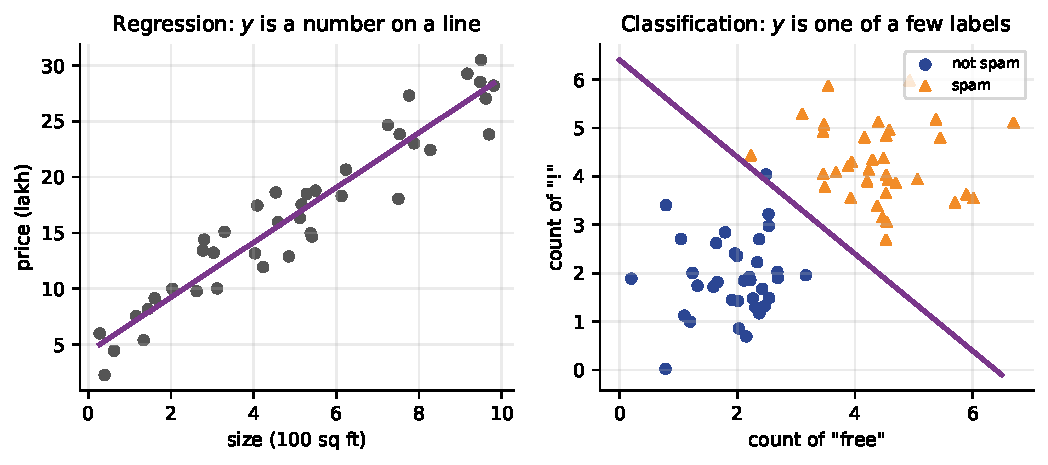
\includegraphics[width=\textwidth]{regvsclf}
\caption{Left: regression, where the target is a number and the model draws a
line (or surface) through the data. Right: classification, where the target is
one of a few labels and the model draws a boundary between them.}
\end{figure}

\begin{itemize}[leftmargin=*]
  \item \textbf{Regression} --- $y$ is a continuous number. House price, stock
    value, tomorrow's temperature, hours until a machine fails.
    \emph{Unit V; lab experiments 3--4.}
  \item \textbf{Classification} --- $y$ is one of a finite set of categories.
    Spam or not spam; digit 0--9; benign or malignant.
    \emph{Unit VI; lab experiments 5--9 and 11--12.}
\end{itemize}

The distinction is about the \emph{target}, not about the features or the
method. The same features can support both: given a patient's measurements you
might predict their blood pressure (regression) or whether they are hypertensive
(classification).

\subsection{A supervised algorithm you can run in your head}

Before any library, here is a complete supervised algorithm.
\textbf{$k$-nearest neighbours} makes a prediction for a new point by finding
the $k$ training points closest to it and taking a vote.

\begin{worked}[1-nearest neighbour, by hand]
Five training flowers, described by (petal length, petal width) in cm:

\begin{center}
\begin{tabular}{@{}ccl@{}}
\toprule
\textbf{petal length} & \textbf{petal width} & \textbf{species}\\
\midrule
1.4 & 0.2 & setosa\\
1.3 & 0.2 & setosa\\
4.7 & 1.4 & versicolor\\
4.5 & 1.5 & versicolor\\
6.0 & 2.5 & virginica\\
\bottomrule
\end{tabular}
\end{center}

A new flower measures $(4.6,\ 1.4)$. Which species does 1-NN predict?

Compute the Euclidean distance $\sqrt{(a_1-b_1)^2 + (a_2-b_2)^2}$ to each:

\begin{center}
\begin{tabular}{@{}llr@{}}
\toprule
\textbf{Training point} & \textbf{Working} & \textbf{Distance}\\
\midrule
$(1.4, 0.2)$ & $\sqrt{3.2^2 + 1.2^2} = \sqrt{10.24 + 1.44}$ & $3.42$\\
$(1.3, 0.2)$ & $\sqrt{3.3^2 + 1.2^2} = \sqrt{10.89 + 1.44}$ & $3.51$\\
$(4.7, 1.4)$ & $\sqrt{0.1^2 + 0.0^2} = \sqrt{0.01}$ & $\mathbf{0.10}$\\
$(4.5, 1.5)$ & $\sqrt{0.1^2 + 0.1^2} = \sqrt{0.02}$ & $0.14$\\
$(6.0, 2.5)$ & $\sqrt{1.4^2 + 1.1^2} = \sqrt{1.96 + 1.21}$ & $1.78$\\
\bottomrule
\end{tabular}
\end{center}

The nearest is $(4.7, 1.4)$ at distance $0.10$, so 1-NN predicts
\textbf{versicolor}. With $k=3$ the three nearest are versicolor, versicolor and
virginica --- the vote is 2--1, and the answer is versicolor again.

\textbf{Two things to notice.} First, this algorithm has no ``training'' in any
meaningful sense: it just stores the data and does all its work at prediction
time. Second, the whole method rests on \emph{distance}, which is why
Section~\ref{sec:pipelines} makes such a fuss about the scale of your features.
\end{worked}

Here is the same computation in NumPy, so you can check your arithmetic:

\begin{lstlisting}
import numpy as np
train = np.array([[1.4,0.2],[1.3,0.2],[4.7,1.4],[4.5,1.5],[6.0,2.5]])
new   = np.array([4.6, 1.4])
d = np.sqrt(((train - new)**2).sum(axis=1))
print(np.round(d, 2))
print("nearest row:", d.argmin())
\end{lstlisting}
\begin{codeout}
[3.42 3.51 0.1  0.14 1.78]
nearest row: 2
\end{codeout}

\subsection{Unsupervised learning}

Here there is no $y$ at all. You have observations and want to know what
structure is in them.

\begin{itemize}[leftmargin=*]
  \item \textbf{Clustering} --- group similar records. Customer segments,
    disease subtypes, document topics. \emph{Unit VII; lab experiment 13.}
  \item \textbf{Dimensionality reduction} --- describe the data with fewer
    features while keeping most of the information. \emph{Unit IV.}
  \item \textbf{Anomaly detection} --- identify observations that do not fit the
    pattern. Fraud, equipment faults. \emph{Lab experiment 10.}
\end{itemize}

\begin{caution}[Unsupervised results are harder to judge]
With no ground truth there is nothing to compute an accuracy against. If a
clustering splits your customers into four groups, no one can tell you whether
those are the ``right'' four groups --- there is no right. Evaluating a
clustering is genuinely harder than evaluating a classifier, and Unit VII spends
real time on it.
\end{caution}

\subsection{Reinforcement learning}

An agent takes actions in an environment and receives a reward. It is never told
the correct action; it only observes consequences, and those consequences are
often delayed --- a chess move's value may not be apparent for thirty moves.
Used in robotics, game playing, control systems and recommendation with
feedback. We cover it here only so you can recognise it; it is not examined
beyond the distinction.

\subsection{Naming the problem}

The skill this section is really teaching is classifying an unfamiliar problem.
Cover the two right-hand columns and try each row.

\begin{center}
\begin{tabular}{@{}p{7.4cm}ll@{}}
\toprule
\textbf{Situation} & \textbf{Family} & \textbf{Task}\\
\midrule
10\,000 past loans marked repaid or defaulted; score a new applicant
  & supervised & classification\\[3pt]
Five years of daily sales; forecast next month
  & supervised & regression\\[3pt]
50\,000 customer records, no labels; find natural groups
  & unsupervised & clustering\\[3pt]
Card transactions; flag the unusual ones
  & unsupervised & anomaly detection\\[3pt]
A warehouse robot that must learn a route
  & reinforcement & policy learning\\
\bottomrule
\end{tabular}
\end{center}

Row four repays thought. Fraud detection \emph{could} be supervised --- if you
had a reliable label for every past transaction. In practice you do not:
confirmed fraud is rare, arrives months late, and is itself biased by whatever
detection system was running at the time. So a problem that is supervised in
principle is often unsupervised in practice, and the reason is operational
rather than mathematical.

\newpage
% =========================================================================
\section{The central difficulty: generalisation}
\label{sec:general}

\subsection{Fitting the training data is trivial}

Here is a model that achieves 100\% accuracy on any training set: store every
training example, and when asked to predict, look up the answer. Perfect score,
zero learning. It has memorised, and it will fail completely on anything it has
not seen.

\begin{keyidea}
The goal is never to fit the data you have. It is to be right about data you
have never seen. That property is called \textbf{generalisation}, and everything
in the rest of this course --- splits, cross-validation, regularization --- is
machinery for estimating it or improving it.
\end{keyidea}

\subsection{Holding data back}

Since we cannot see the future, we simulate it: hide some of the data from the
model, then use that hidden part to estimate how it will behave on genuinely new
cases.

\begin{figure}[h]
\centering
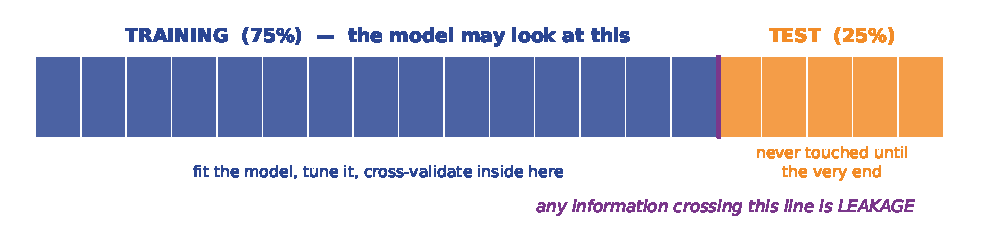
\includegraphics[width=\textwidth]{split}
\caption{The train/test split. The model may look at the blue part as often as
it likes. The orange part is opened once, at the very end, to produce the number
you report.}
\end{figure}

\begin{caution}[The test set is not a tuning signal]
If you try twenty models and pick the one with the best test score, that score
is no longer an honest estimate --- you have used the test set to make a choice,
so it has leaked into your decision. The honest procedure is to split three ways
(train / validation / test), tune on validation, and touch the test set once.
Cross-validation, below, is a cheaper version of the same idea.
\end{caution}

\subsection{Overfitting, seen properly}

Let us watch a model overfit. We generate 30 points from a gentle curve plus
noise, hold out 40\%, and fit polynomials of increasing degree.

\begin{figure}[h]
\centering
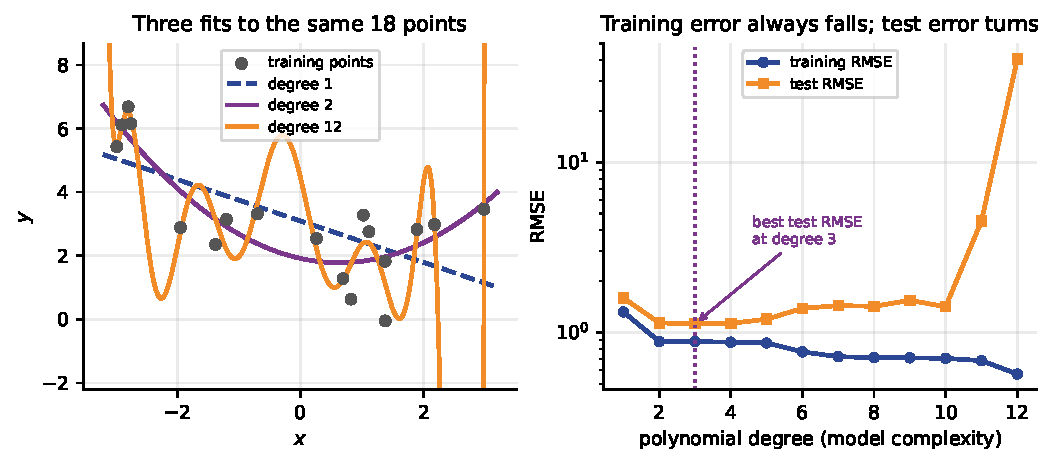
\includegraphics[width=\textwidth]{overfitting}
\caption{Left: a straight line under-fits, a parabola fits well, and a
degree-12 polynomial contorts itself through every training point. Right: the
same experiment measured. Training error falls monotonically as complexity
increases; test error falls, bottoms out, then explodes.}
\end{figure}

The measured numbers behind that right-hand panel:

\begin{center}
\begin{tabular}{@{}lrr@{}}
\toprule
\textbf{Model} & \textbf{Training RMSE} & \textbf{Test RMSE}\\
\midrule
Degree 1 (straight line)   & 1.32 & 1.60\\
Degree 2 (parabola)        & 0.89 & 1.14\\
Degree 3 (best test error) & 0.86 & 1.10\\
Degree 12                  & \textbf{0.57} & \textbf{40.52}\\
\bottomrule
\end{tabular}
\end{center}

Read the last row carefully. The degree-12 model is the \emph{best} model by
training error and catastrophically the worst by test error --- off by 40 units
where the data spans about 10. If you had judged it on training error you would
have shipped the worst possible choice.

\begin{keyidea}
\textbf{The gap between training and test error is the diagnostic.} A small gap
with both errors high means under-fitting: the model is too simple. A tiny
training error with a large test error means over-fitting: the model has learned
the noise. You want the point where test error is lowest, which is usually
\emph{not} where training error is lowest.
\end{keyidea}

\subsection{Cross-validation}

A single split has a problem: with a small dataset, which rows happen to land in
the test set moves the answer around. Iris has 150 rows, so a 25\% test set is
38 flowers; two flowers changing sides moves accuracy by five points.

$k$-fold cross-validation fixes this. Split the data into $k$ equal folds; train
on $k-1$ of them and test on the one left out; repeat $k$ times so each fold
serves as the test set once; average.

\begin{lstlisting}
from sklearn.model_selection import cross_val_score
scores = cross_val_score(model, X, y, cv=10)
print(scores.round(3))
print(f"mean {scores.mean():.3f}  sd {scores.std():.3f}")
\end{lstlisting}
\begin{codeout}
[1.    0.933 1.    0.933 0.867 0.933 0.867 1.    1.    1.   ]
mean 0.953  sd 0.052
\end{codeout}

Look at the spread: individual folds range from 0.867 to 1.000. Reporting
``97.4\% accuracy'' from one lucky split would have been true and misleading.
The honest summary is $0.953 \pm 0.052$.

\begin{caution}[Quote the spread]
A single accuracy figure with no measure of variability is nearly meaningless on
a small dataset. Get into the habit of reporting mean and standard deviation
across folds, and of not quoting more significant figures than your spread
justifies. ``95\%'' is honest here; ``95.33\%'' is not.
\end{caution}

\subsection{Data leakage}
\label{sec:leakage}

\textbf{Data leakage} is the use, at training time, of information that would
not be available at prediction time. It is the single most common way to get a
wonderful result that means nothing, and it is subtle enough that it catches
professionals.

The clearest demonstration uses data with \emph{no signal at all}. We generate
100 rows of 5000 pure-noise features and assign labels by coin flip. Nothing is
predictable; the honest accuracy of any model is 50\%.

\begin{lstlisting}
import numpy as np
from sklearn.feature_selection import SelectKBest, f_classif
from sklearn.model_selection import cross_val_score
from sklearn.neighbors import KNeighborsClassifier
from sklearn.pipeline import make_pipeline

rng = np.random.default_rng(0)
X = rng.normal(size=(100, 5000))      # pure noise
y = rng.integers(0, 2, 100)           # coin flips

# WRONG: pick the 20 "best" features using every row, including the test rows
Xsel  = SelectKBest(f_classif, k=20).fit_transform(X, y)
wrong = cross_val_score(KNeighborsClassifier(3), Xsel, y, cv=10).mean()

# RIGHT: selection lives inside the pipeline, so it happens inside each fold
pipe  = make_pipeline(SelectKBest(f_classif, k=20), KNeighborsClassifier(3))
right = cross_val_score(pipe, X, y, cv=10).mean()

print(f"selection before the split : {wrong:.2f}")
print(f"selection inside the fold  : {right:.2f}")
\end{lstlisting}
\begin{codeout}
selection before the split : 0.81
selection inside the fold  : 0.50
\end{codeout}

Eighty-one percent accuracy on random noise. The feature selector examined all
5000 columns \emph{including the test rows' labels} and picked the twenty that
happened to correlate with $y$ by chance. Those twenty then looked predictive
during cross-validation, because the selection had already peeked.

\begin{keyidea}
Any step that \emph{learns something from the data} --- scaling, imputation,
feature selection, encoding --- must be fitted on the training portion only. The
practical rule that makes this automatic is: \textbf{put every such step inside
a \texttt{Pipeline}} and let scikit-learn handle the fold boundaries.
\end{keyidea}

\newpage
% =========================================================================
\section{NumPy: the foundation}

\subsection{The \texttt{ndarray}}

NumPy provides one central object: the $n$-dimensional array. Unlike a Python
list, every element has the same type and the whole thing sits in one contiguous
block of memory. That is what makes it fast, and it is why every other library
in the stack is built on it.

\begin{lstlisting}
import numpy as np
a = np.array([[1, 2, 3],
              [4, 5, 6]])
print(a.shape, a.dtype)
print(a.sum(axis=0))       # down the columns
print(a.sum(axis=1))       # across the rows
\end{lstlisting}
\begin{codeout}
(2, 3) int64
[5 7 9]
[ 6 15]
\end{codeout}

The \texttt{axis} argument confuses everybody at first. The rule:
\texttt{axis=0} collapses the rows (giving one value per column);
\texttt{axis=1} collapses the columns (one value per row). Say ``the axis I name
is the one that disappears''.

\subsection{Vectorisation, and why it matters}

Consider computing the mean squared error between predictions and truth. Written
as a loop:

\begin{lstlisting}
total = 0.0
for i in range(len(y)):
    d = y[i] - yhat[i]
    total += d * d
mse = total / len(y)
\end{lstlisting}

Written with NumPy:

\begin{lstlisting}
mse = np.mean((y - yhat) ** 2)
\end{lstlisting}

The second is shorter, but the important difference is speed. Timed on one
million elements:

\begin{codeout}
loop  :    162.9 ms
numpy :      1.85 ms
ratio :       88x
\end{codeout}

The loop runs in the Python interpreter, one element at a time, with all the
overhead that implies. The NumPy version dispatches to compiled C which walks a
contiguous block. The gap widens with array size.

\begin{keyidea}
You have just written the \textbf{Mean Squared Error}, the first loss function
of Unit II. Every optimiser in Unit III exists to make that number smaller. The
whole course is, in a sense, an elaboration of \texttt{np.mean((y - yhat)**2)}.
\end{keyidea}

\begin{worked}[MSE, MAE and RMSE by hand]
Three predictions. True values $y = (3, 1, 4)$, predictions
$\hat{y} = (2.5,\ 1.5,\ 4.5)$.

Errors: $y - \hat{y} = (0.5,\ -0.5,\ -0.5)$.

\[
\text{MAE} = \frac{|0.5| + |{-0.5}| + |{-0.5}|}{3} = \frac{1.5}{3} = 0.5
\]
\[
\text{MSE} = \frac{0.5^2 + (-0.5)^2 + (-0.5)^2}{3} = \frac{0.75}{3} = 0.25
\]
\[
\text{RMSE} = \sqrt{0.25} = 0.5
\]

Verify:
\begin{lstlisting}
y    = np.array([3.0, 1.0, 4.0])
yhat = np.array([2.5, 1.5, 4.5])
print("MAE ", np.mean(np.abs(y - yhat)))
print("MSE ", np.mean((y - yhat)**2))
print("RMSE", np.sqrt(np.mean((y - yhat)**2)))
\end{lstlisting}
\begin{codeout}
MAE  0.5
MSE  0.25
RMSE 0.5
\end{codeout}

MAE and RMSE agree here only because every error has the same magnitude. Change
the first prediction to $\hat{y}_1 = 0$, so the errors become $(3, -0.5, -0.5)$,
and recompute:

\[
\text{MAE} = \frac{3 + 0.5 + 0.5}{3} = 1.333,
\qquad
\text{RMSE} = \sqrt{\frac{9 + 0.25 + 0.25}{3}} = \sqrt{3.167} = 1.780
\]

RMSE is now a third larger than MAE, because squaring punishes the one big error
far more than the two small ones. That asymmetry is exactly why the choice of
loss function matters --- and it is the subject of Unit II.
\end{worked}

\subsection{Broadcasting and boolean masks}

Two more NumPy ideas you will use constantly.

\textbf{Broadcasting} lets arrays of different shapes combine, by stretching the
smaller one:

\begin{lstlisting}
X = np.array([[1., 2.], [3., 4.], [5., 6.]])
col_means = X.mean(axis=0)        # shape (2,)
print(col_means)
print(X - col_means)              # (3,2) - (2,) works: broadcast down the rows
\end{lstlisting}
\begin{codeout}
[3. 4.]
[[-2. -2.]
 [ 0.  0.]
 [ 2.  2.]]
\end{codeout}

You have just centred a dataset --- the first half of what \texttt{StandardScaler}
does.

\textbf{Boolean masks} select without loops:

\begin{lstlisting}
v = np.array([3, 8, 1, 9, 4])
print(v > 4)
print(v[v > 4])
print((v > 4).sum())      # True counts as 1: how many exceed 4
\end{lstlisting}
\begin{codeout}
[False  True False  True False]
[8 9]
2
\end{codeout}

\newpage
% =========================================================================
\section{pandas: tabular data}

Where NumPy gives you a grid of numbers, pandas gives you a table with column
names, mixed types, and a notion of missing data. That is what real datasets
look like.

\subsection{The first four calls, every time}

Before you model anything, run these four. They take five seconds and answer
most of the questions you would otherwise discover painfully later.

\begin{lstlisting}
import pandas as pd
from sklearn.datasets import load_iris

d  = load_iris(as_frame=True)
df = d.frame
df.head(3)
\end{lstlisting}
\begin{codeout}
   sepal length (cm)  sepal width (cm)  petal length (cm)  petal width (cm)  target
0                5.1               3.5                1.4               0.2       0
1                4.9               3.0                1.4               0.2       0
2                4.7               3.2                1.3               0.2       0
\end{codeout}

\begin{lstlisting}
df.describe().round(2)
\end{lstlisting}
\begin{codeout}
       sepal length (cm)  sepal width (cm)  petal length (cm)  petal width (cm)  target
count             150.00            150.00             150.00            150.00  150.00
mean                5.84              3.06               3.76              1.20    1.00
std                 0.83              0.44               1.77              0.76    0.82
min                 4.30              2.00               1.00              0.10    0.00
25%                 5.10              2.80               1.60              0.30    0.00
50%                 5.80              3.00               4.35              1.30    1.00
75%                 6.40              3.30               5.10              1.80    2.00
max                 7.90              4.40               6.90              2.50    2.00
\end{codeout}

Read that table rather than skipping it. Petal length has a standard deviation of
1.77 while petal width has 0.76 --- more than double. Sepal width ranges over
2.4\,cm while petal length ranges over 5.9\,cm. Those differences will matter
enormously in Section~\ref{sec:pipelines}.

The other two calls:

\begin{lstlisting}
df.info()              # dtypes and non-null counts: finds text stored as numbers
df.isna().sum()        # missing values per column
\end{lstlisting}

\begin{keyidea}
\texttt{head}, \texttt{info}, \texttt{describe}, \texttt{isna().sum()}. Build
the habit now. Unit IV is the disciplined, systematic version of this reflex,
and lab experiment 2 assesses it.
\end{keyidea}

\subsection{Selecting, creating and grouping}

\begin{lstlisting}
df["petal ratio"] = df["petal length (cm)"] / df["petal width (cm)"]
print(df.groupby("target")["petal ratio"].mean().round(2))
\end{lstlisting}
\begin{codeout}
target
0    6.91
1    3.24
2    2.78
Name: petal ratio, dtype: float64
\end{codeout}

That one line has done something useful: it shows setosa (target 0) has petals
more than twice as long as they are wide relative to the others, which is
precisely why it separates so cleanly in the figure below. Creating a feature
like this from domain reasoning is called \textbf{feature engineering}, and it
is Unit IV.

\begin{figure}[h]
\centering
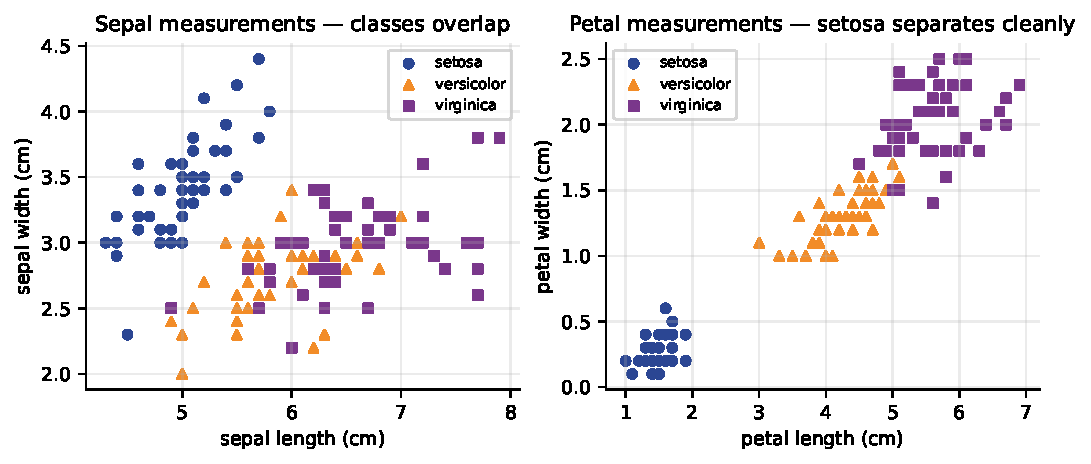
\includegraphics[width=\textwidth]{iris}
\caption{The Iris data in two different feature pairs. Sepal measurements
(left) leave the three species overlapping. Petal measurements (right) separate
setosa completely and leave only versicolor and virginica touching. Choosing
which features to use is often worth more than choosing which model to use.}
\end{figure}

\newpage
% =========================================================================
\section{scikit-learn: one API for every model}
\label{sec:pipelines}

\subsection{The estimator interface}

Every model in scikit-learn --- and there are hundreds --- exposes the same
three methods:

\begin{lstlisting}
est.fit(X, y)        # learn from data
est.predict(X)       # apply to new data
est.score(X, y)      # evaluate
\end{lstlisting}

Every transformer exposes:

\begin{lstlisting}
tr.fit(X)            # learn the transformation (e.g. the mean and sd)
tr.transform(X)      # apply it
tr.fit_transform(X)  # both, for convenience - on TRAINING data only
\end{lstlisting}

This uniformity is the library's central design decision, and it pays off
immediately: swapping a $k$-nearest-neighbours classifier for a support vector
machine changes one line and nothing else. Learn the interface once here and
every model in Units V--VII is already familiar.

\subsection{An entire workflow in twelve lines}

\begin{lstlisting}
from sklearn.datasets import load_iris
from sklearn.model_selection import train_test_split
from sklearn.preprocessing import StandardScaler
from sklearn.neighbors import KNeighborsClassifier
from sklearn.pipeline import make_pipeline

X, y = load_iris(return_X_y=True)
X_train, X_test, y_train, y_test = train_test_split(
    X, y, test_size=0.25, random_state=0, stratify=y)

model = make_pipeline(StandardScaler(), KNeighborsClassifier(n_neighbors=5))
model.fit(X_train, y_train)
print("test accuracy:", model.score(X_test, y_test))
\end{lstlisting}
\begin{codeout}
test accuracy: 0.9736842105263158
\end{codeout}

Each argument is doing a job:

\begin{itemize}[leftmargin=*]
  \item \texttt{test\_size=0.25} holds back 38 of the 150 flowers.
  \item \texttt{random\_state=0} fixes the shuffle so you and I get the same
    split. Without it, every run gives a different answer and nothing is
    reproducible.
  \item \texttt{stratify=y} keeps the class proportions the same in both halves.
    Without it a random split can, by bad luck, give you a test set with too few
    of one species.
  \item \texttt{make\_pipeline} chains the scaler and the model into one object,
    so the scaler is fitted \emph{inside} the training portion only. This is the
    leak-proof construction from Section~\ref{sec:leakage}.
\end{itemize}

Look at what the model actually got right and wrong:

\begin{lstlisting}
from sklearn.metrics import confusion_matrix
print(confusion_matrix(y_test, model.predict(X_test)))
\end{lstlisting}
\begin{codeout}
                 pred setosa  pred versicolor  pred virginica
true setosa               13                0               0
true versicolor            0               13               0
true virginica             0                1              11
\end{codeout}

One error in 38: a virginica called versicolor. That is exactly the pair the
figure showed touching, so the model failed precisely where the data is
genuinely ambiguous. A confusion matrix tells you \emph{which} mistakes are
made; an accuracy figure never does.

\subsection{Why the pipeline is not optional}

Section~\ref{sec:leakage} argued for pipelines on correctness grounds. Here is
the other argument: without scaling, distance-based models can fail completely.

We construct a deliberately unfair dataset --- one feature that determines the
class, on a range of 0--1, and one pure-noise feature on a range of 0--10\,000:

\begin{figure}[h]
\centering
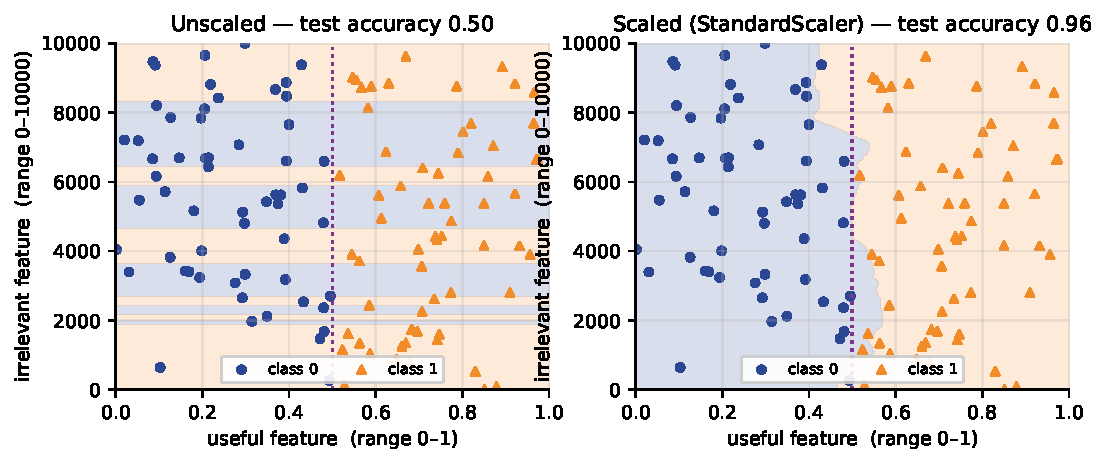
\includegraphics[width=\textwidth]{scaling}
\caption{The same KNN classifier on the same data. Left, unscaled: the
irrelevant feature's huge numeric range dominates the distance calculation, the
decision regions run horizontally, and accuracy is 0.50 --- pure chance. Right,
with \texttt{StandardScaler} inside the pipeline: the boundary is vertical,
following the feature that actually matters, and accuracy is 0.96.}
\end{figure}

\begin{center}
\begin{tabular}{@{}lr@{}}
\toprule
\textbf{Model} & \textbf{Test accuracy}\\
\midrule
\texttt{KNeighborsClassifier(5)} on raw features & 0.50\\
\texttt{make\_pipeline(StandardScaler(), KNeighborsClassifier(5))} & \textbf{0.96}\\
\bottomrule
\end{tabular}
\end{center}

The reason is arithmetic. Euclidean distance squares the difference in each
feature and adds. A difference of 3000 in the noise feature contributes
$9{,}000{,}000$; a difference of 0.5 in the useful feature contributes $0.25$.
The useful feature is not slightly outweighed --- it is invisible.

\begin{keyidea}
Any method that measures distance (KNN, SVM with RBF kernel, K-means) or that
uses gradient descent (Units II--III) needs features on comparable scales. Tree
based methods do not, because they split one feature at a time. Knowing which
camp a method is in tells you whether scaling is optional.
\end{keyidea}

\subsection{Choosing a hyperparameter}

$k$ in KNN is a \textbf{hyperparameter}: a setting you choose, not a value the
model learns. Choose it by measurement, not by taste.

\begin{lstlisting}
for k in (1, 3, 5, 7, 9, 15, 25, 50):
    m = make_pipeline(StandardScaler(), KNeighborsClassifier(k))
    print(f"k={k:<3} cv accuracy {cross_val_score(m, X, y, cv=10).mean():.3f}")
\end{lstlisting}
\begin{codeout}
k=1   cv accuracy 0.953
k=3   cv accuracy 0.953
k=5   cv accuracy 0.953
k=7   cv accuracy 0.953
k=9   cv accuracy 0.953
k=15  cv accuracy 0.960
k=25  cv accuracy 0.947
k=50  cv accuracy 0.880
\end{codeout}

Two lessons. First, performance is flat from $k=1$ to $k=9$ --- on this easy
dataset the choice barely matters, and a student who reports ``I tuned $k$ and
got a big improvement'' has probably fooled themselves. Second, at $k=50$
accuracy collapses: with only 50 flowers per species, a 50-neighbour vote
inevitably reaches across class boundaries. Both failure modes ($k$ too small
fits noise, $k$ too large smooths across classes) are visible in one table.

\subsection{More data or a better model?}

A common instinct when a model underperforms is to try a fancier model. Often
the right answer is more data --- and you can find out which, by plotting a
learning curve.

\begin{figure}[h]
\centering
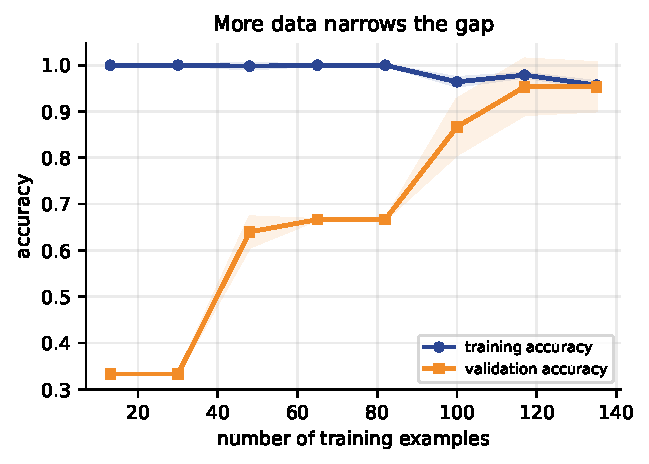
\includegraphics[width=0.62\textwidth]{learningcurve}
\caption{Accuracy against training-set size for KNN on Iris. The two curves have
essentially converged by 120 examples, which says that adding more Iris flowers
would not help. When the curves are still far apart at the right-hand edge, more
data is the cheapest improvement available.}
\end{figure}

\newpage
% =========================================================================
\section{Summary}

\begin{itemize}[leftmargin=*]
  \item Machine learning suits problems where you have \textbf{examples of the
    answer} but cannot \textbf{state the rule}.
  \item Mitchell's $T$, $P$, $E$ forces you to name the performance measure
    before you model. Most project failures are $P$ failures.
  \item Three families: \textbf{supervised} (regression, classification),
    \textbf{unsupervised} (clustering, dimensionality reduction, anomaly
    detection), \textbf{reinforcement} (a policy learned from reward).
  \item The goal is never to fit the training data --- it is to generalise. The
    \textbf{gap} between training and test error is your diagnostic.
  \item A single split on a small dataset is unreliable. Cross-validate, and
    quote the spread.
  \item \textbf{Data leakage} produced 81\% accuracy on pure noise. Put every
    fitted step inside a \texttt{Pipeline}.
  \item \textbf{NumPy} $\rightarrow$ \textbf{pandas} $\rightarrow$
    \textbf{scikit-learn}, with one \texttt{fit}/\texttt{predict} interface for
    every model.
  \item Distance-based and gradient-based methods need scaling. Trees do not.
\end{itemize}

\textbf{Next (L2): loss functions.} We put a number on how wrong a prediction
is --- MSE, MAE and Huber for regression, cross-entropy for classification,
hinge and triplet for margins. Everything in Units V--VII minimises one of them.

\newpage
% =========================================================================
\section{Practice questions}
\label{sec:practice}

Attempt these before reading Section~\ref{sec:solutions}.

\begin{enumerate}[leftmargin=*, label=\textbf{Q\arabic*.}]

\item State Mitchell's $T$, $P$ and $E$ for a system that recommends films to a
streaming subscriber.

\item\label{ex:hospital} A hospital wants to predict which patients will miss an
appointment. Which of the five cautions in Section~\ref{sec:cautions} is most
likely to bite, and why?

\item Classify each as supervised regression, supervised classification,
unsupervised, or reinforcement:
\begin{enumerate}[label=(\alph*)]
  \item predicting tomorrow's electricity demand;
  \item grouping news articles by topic with no labels;
  \item deciding whether a transaction is fraudulent, given past confirmed fraud;
  \item tuning a thermostat rewarded for comfort and penalised for energy use.
\end{enumerate}

\item Using the five training flowers from the worked example in
Section~\ref{sec:families}, predict the species of a flower measuring
$(1.5,\ 0.3)$ using 1-NN. Show the distances.

\item A colleague reports 99\% accuracy on a medical test set. What three
questions would you ask before believing it?

\item Rewrite this loop using NumPy, and name the quantity it computes:
\begin{lstlisting}
s = 0
for i in range(len(a)):
    s += abs(a[i] - b[i])
result = s / len(a)
\end{lstlisting}

\item Explain, in terms of Euclidean distance, why the unscaled classifier in
Section~\ref{sec:pipelines} scored exactly 0.50.

\item In the overfitting table, degree 12 had the lowest training RMSE of all.
Why is that not a reason to prefer it?

\item Your cross-validation gives folds
$[0.95, 0.93, 0.97, 0.62, 0.96]$. What should you investigate, and why is
reporting the mean alone inadequate?

\item Why does \texttt{make\_pipeline(StandardScaler(), KNN())} give an honest
cross-validation score when scaling the whole array first does not?

\end{enumerate}

% =========================================================================
\section{Solutions}
\label{sec:solutions}

\begin{enumerate}[leftmargin=*, label=\textbf{Q\arabic*.}]

\item $T$: recommend a film for a given subscriber. $E$: past viewing and
ratings history. $P$: a stated, measurable quantity such as click-through rate
on recommendations, or watch-time of recommended titles. Any defensible $P$ is
acceptable \emph{provided it is named explicitly and could actually be
measured} --- ``user satisfaction'' is not a performance measure until you say
how you would compute it.

\item Most likely caution 5, \textbf{distribution shift}. Appointment-attendance
behaviour depends on clinic policy, transport, weather and season, all of which
change; a model trained on last year degrades. Caution 4 (explainability) is
also defensible if the prediction is used to allocate scarce appointments, since
a patient denied a slot may reasonably demand a reason. Caution 3 deserves a
mention too: the cost of wrongly predicting attendance is not symmetric.

\item (a) supervised regression; (b) unsupervised clustering; (c) supervised
classification; (d) reinforcement learning.

\item Distances from $(1.5, 0.3)$:
$(1.4,0.2) \rightarrow \sqrt{0.01+0.01} = 0.14$;
$(1.3,0.2) \rightarrow \sqrt{0.04+0.01} = 0.22$;
$(4.7,1.4) \rightarrow \sqrt{10.24+1.21} = 3.38$;
$(4.5,1.5) \rightarrow \sqrt{9.0+1.44} = 3.23$;
$(6.0,2.5) \rightarrow \sqrt{20.25+4.84} = 5.01$.
Nearest is $(1.4,0.2)$ at $0.14$, so 1-NN predicts \textbf{setosa}.

\item Reasonable questions: (i) What is the base rate --- if 99\% of patients are
healthy, 99\% accuracy is what you get by predicting ``healthy'' every time.
(ii) How was the test set constructed, and did any preprocessing see it?
(iii) What is the recall on the positive class --- how many sick patients were
missed? Also good: how many test cases were there, and is the test set from the
same hospital and equipment as deployment?

\item \texttt{result = np.mean(np.abs(a - b))}. It is the \textbf{Mean Absolute
Error}, which we meet again in Unit II.

\item Euclidean distance squares each feature's difference and sums. The noise
feature spans 0--10\,000, so typical squared differences are of order $10^6$--$10^7$;
the useful feature spans 0--1, contributing at most 1. The sum is therefore
determined almost entirely by the noise feature, so the ``nearest'' neighbours
are those with similar noise values, which carry no class information. The
result is a coin flip, hence 0.50.

\item Because training error measures how well the model reproduces data it has
already seen, which a sufficiently flexible model can always do perfectly. It
says nothing about new data. The degree-12 model's test RMSE was 40.52 against
1.10 for degree 3 --- it is the worst model available, and training error ranked
it best.

\item Investigate the fourth fold. A single fold far below the others suggests
either that the folds are not comparable (an unstratified split leaving one fold
with an unusual class mix), or that a cluster of genuinely hard or mislabelled
cases landed together. Reporting only the mean (0.886) hides the instability;
the standard deviation (0.135) is the signal that something is wrong.

\item Because \texttt{cross\_val\_score} refits the \emph{whole pipeline} inside
each fold. The scaler's mean and standard deviation are computed from that
fold's training rows only, so the held-out rows contribute nothing to the
transformation. Scaling the full array first computes those statistics from
every row, including the ones about to be used for evaluation --- so the model is
tested on data whose statistics it has already absorbed.

\end{enumerate}

\newpage
% =========================================================================
\section{References and further reading}

All links were checked on 4 August 2026. Free and no-login resources are marked
\textbf{[free]}.

\subsection*{Textbooks}

\begin{itemize}[leftmargin=*]
  \item M\"uller, A.\ C.\ and Guido, S. \emph{Introduction to Machine Learning
    with Python}. O'Reilly, 2016. \textbf{Chapter 1} --- prescribed text; the
    Iris walkthrough there is the same one used in these notes.
  \item Bishop, C.\ M. \emph{Pattern Recognition and Machine Learning}.
    Springer, 2006. \textbf{Chapter 1, \S1.1} --- the polynomial curve-fitting
    example, which is the classical treatment of over-fitting.
    \textbf{[free]} from Microsoft Research.
  \item James, G., Witten, D., Hastie, T., Tibshirani, R.\ and Taylor, J.
    \emph{An Introduction to Statistical Learning with Python}. Springer, 2023.
    \textbf{Chapters 1--2}. \textbf{[free]} \url{https://www.statlearning.com/}
  \item Murphy, K.\ P. \emph{Probabilistic Machine Learning: An Introduction}.
    MIT Press, 2022. \textbf{Chapter 1} --- an excellent taxonomy of learning
    problems. \textbf{[free]} \url{https://probml.github.io/pml-book/book1.html}
  \item VanderPlas, J. \emph{Python Data Science Handbook}. O'Reilly.
    \textbf{[free]} in full online ---
    \url{https://jakevdp.github.io/PythonDataScienceHandbook/}
\end{itemize}

\subsection*{Online courses}

\begin{itemize}[leftmargin=*]
  \item \textbf{NPTEL --- Introduction to Machine Learning}, Prof.\ Balaraman
    Ravindran, IIT Madras. The closest match to this syllabus, in Indian
    academic idiom, and free to audit. \textbf{[free]}\\
    \url{https://nptel.ac.in/courses/106106139}\\
    Course preview and enrolment:
    \url{https://onlinecourses.nptel.ac.in/noc23_cs18/preview}\\
    Prof.\ Ravindran's index of NPTEL courses:
    \url{https://www.cse.iitm.ac.in/~ravi/nptel-courses/}
  \item \textbf{SWAYAM} --- the national portal hosting NPTEL and other Indian
    university courses. \textbf{[free]} \url{https://swayam.gov.in/}
  \item \textbf{Google Machine Learning Crash Course} --- short, practical, with
    interactive exercises. Good for the vocabulary in this lecture.
    \textbf{[free]}
    \url{https://developers.google.com/machine-learning/crash-course}
  \item \textbf{Kaggle Learn --- Intro to Machine Learning} --- four hours,
    entirely hands-on, runs in the browser with no installation.
    \textbf{[free]} \url{https://www.kaggle.com/learn/intro-to-machine-learning}
\end{itemize}

\subsection*{Videos}

\begin{itemize}[leftmargin=*]
  \item StatQuest with Josh Starmer, \emph{A Gentle Introduction to Machine
    Learning} (about 12 minutes). The clearest short explanation of training
    versus testing that exists. \textbf{[free]} \url{https://youtu.be/Gv9_4yMHFhI}
  \item StatQuest, \emph{Machine Learning Fundamentals: Bias and Variance}.
    Watch this before Unit V. \textbf{[free]} \url{https://youtu.be/EuBBz3bI-aA}
  \item StatQuest, \emph{Machine Learning Fundamentals: Cross Validation} ---
    covers Section~\ref{sec:general} of these notes in six minutes.
    \textbf{[free]} \url{https://youtu.be/fSytzGwwBVw}
  \item StatQuest full video index, organised by topic, useful all semester.
    \textbf{[free]} \url{https://statquest.org/video-index/}
\end{itemize}

\subsection*{Documentation and interactive explainers}

\begin{itemize}[leftmargin=*]
  \item scikit-learn, \emph{Getting Started}. \textbf{[free]}
    \url{https://scikit-learn.org/stable/getting_started.html}
  \item scikit-learn, \emph{Common Pitfalls and Recommended Practices} --- the
    official treatment of leakage and of \texttt{random\_state}. Read this one
    properly; it covers Section~\ref{sec:leakage} in more depth. \textbf{[free]}
    \url{https://scikit-learn.org/stable/common_pitfalls.html}
  \item scikit-learn, \emph{Cross-validation}. \textbf{[free]}
    \url{https://scikit-learn.org/stable/modules/cross_validation.html}
  \item NumPy, \emph{NumPy: the absolute basics for beginners}. \textbf{[free]}
    \url{https://numpy.org/doc/stable/user/absolute_beginners.html}
  \item pandas, \emph{10 minutes to pandas}. \textbf{[free]}
    \url{https://pandas.pydata.org/docs/user_guide/10min.html}
  \item \textbf{MLU-Explain} --- visual, interactive explanations of
    train/test splits, bias--variance and cross-validation from Amazon's machine
    learning university. Genuinely worth an hour. \textbf{[free]}
    \url{https://mlu-explain.github.io/}
\end{itemize}

\subsection*{Articles}

\begin{itemize}[leftmargin=*]
  \item Brownlee, J. \emph{Data Leakage in Machine Learning}, Machine Learning
    Mastery. A practical companion to Section~\ref{sec:leakage}. \textbf{[free]}
    \url{https://machinelearningmastery.com/data-leakage-machine-learning/}
\end{itemize}

\notesources{\AMLUnitISources}

\end{document}
